\chapter{数据库编程}

\section{SQLite数据库的使用}

\url{https://blogs.windows.com/buildingapps/2017/02/06/using-sqlite-databases-uwp-apps/}

For many developers, SQLite has become the preferred client-side technology for data storage. It is a server-less, embedded, open-source database engine that satisfies most local data access scenarios. There are numerous advantages that come with its use, many of which are explained in the SQLite about page.

Since the Windows 10 Anniversary Update (Build 14393), SQLite has also shipped as part of the Windows SDK. This means that when you are building your Universal Windows Platform (UWP) app that runs across the different Windows device form factors, you can take advantage of the SDK version of SQLite for local data storage. This comes with some advantages:

\begin{itemize}
	\item Your application size reduces since you don’t download your own SQLite binary and package it as part of your application 

	\begin{itemize}
		\item Note: \ProgrammingLanguagePackageName{Microsoft.Data.SQLite} (used in the example below) currently has an issue where both SQLite3.dll and WinSQLite.dll are loaded in memory whenever a .NET Native version of your application is run. This is a tracked issue that will be addressed in subsequent updates of the library. 
	\end{itemize}

	\item You can depend on the Windows team to update the version of SQLite running on the operating system with every release of Windows.
	
	\item Application load time has the potential to be faster since the SDK version of SQLite will likely already be loaded in memory.
\end{itemize}

Below, we provided a quick coding example on how to consume the SDK version of SQLite in your C\# application.

Note: Since the Windows SDK version of SQLite has only been available since the Windows 10 Anniversary Update, it can only be used for UWP apps targeting Build 14393 or higher.

\subsection{C\# Example}

In this example, we will build a UWP application that will allow users to input text into an app local database. The goal is to provide developers with concise guidance on how to use the SQLite binary that’s shipped as part of the Windows SDK. Therefore this code sample is meant to be as simple as possible, so as to provide a foundation that can be further built upon.

An example of the end product is shown below:

\begin{figure}
	\centering
	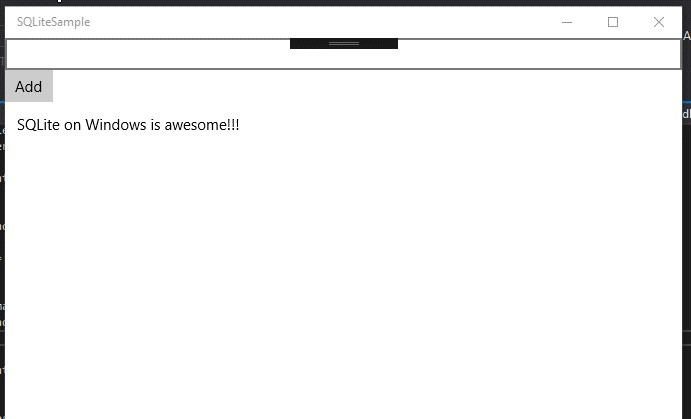
\includegraphics[width=\linewidth]{figures/Sqlite_sample}
	\caption{}
	\label{fig:sqlitesample}
\end{figure}

\subsection{SQLite C\# API Wrappers}

As mentioned in the SQLite documentation, the API provided by SQLite is fairly low-level and can add an additional level of complexity for the developer. Because of this, many open-source libraries have been produced to act as wrappers around the core SQLite API. These libraries abstract away a lot of the core details behind SQLite, allowing developers to more directly deal with executing SQL statements and parsing the results.
For SQLite consumption across Windows, we recommend the open-source Microsoft.Data.Sqlite library built by the ASP.NET team. It is actively being maintained and provides an intuitive wrapper around the SQLite API. The rest of the example assumes use of the Microsoft.Data.Sqlite library.

Alternative SQLite wrappers are also linked in the “Additional Resources” section below.

\subsection{Visual Studio set-up}

The packages used in this sample have a dependency on NuGet version 3.5 or greater. You can check your version of NuGet by going to Help ‣ About Microsoft Visual Studio and looking through the Installed Products for NuGet Package Manager. You can go to the NuGet download page and grab the version 3.5 VSIX update if you have a lower version.

Note: Visual Studio 2015 Update 3 is pre-installed with NuGet version 3.4, and will likely require an upgrade. Visual Studio 2017 RC is installed with NuGet version 4.0, which works fine for this sample.

\subsubsection{Adding \ProgrammingLanguagePackageName{Microsoft.Data.Sqlite} and upgrading the .NET Core template}

The \ProgrammingLanguagePackageName{Microsoft.Data.Sqlite} package relies on at least the 5.2.2 version of .NET Core for UWP, so we’ll begin by upgrading this:

\begin{itemize}
	\item Right click on \SoftwareMenu{References} $ \to $ \SoftwareMenu{Manage NuGet Packages}
	\item Under the \SoftwareMenu{Installed} tab, look for the \ProgrammingLanguagePackageName{Microsoft.NETCore.UniversalWindowsPlatform} package and check the version number on the right-hand side. If it’s not up to date, you’ll be able to update to version 5.2.2 or higher.
\end{itemize}

\begin{figure}
	\centering
	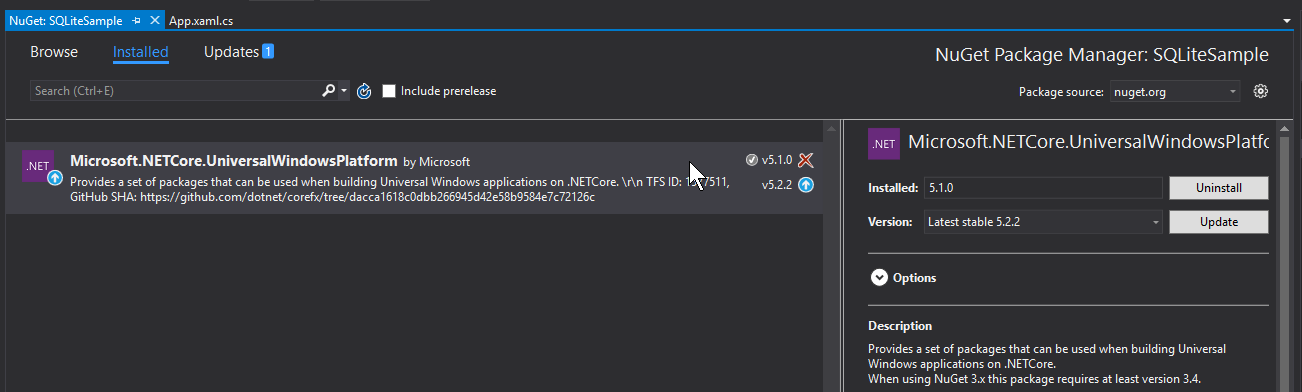
\includegraphics[width=\linewidth]{figures/sqlite_package_check}
	\caption{}
	\label{fig:sqlitepackagecheck}
\end{figure}

Note: Version 5.2.2 is the default for VS 2017 RC. Therefore, this step is not required if you are using this newest version of Visual Studio.

To add the Microsoft.Data.Sqlite NuGet package to your application, follow a similar pattern:

\begin{itemize}
	\item Right-click on \SoftwareMenu{References} $ \to $ \SoftwareMenu{Manage NuGet Packages}
	\item Under the Browse tab, search for the Microsoft.Data.Sqlite package and install it.
\end{itemize}

\begin{figure}
	\centering
	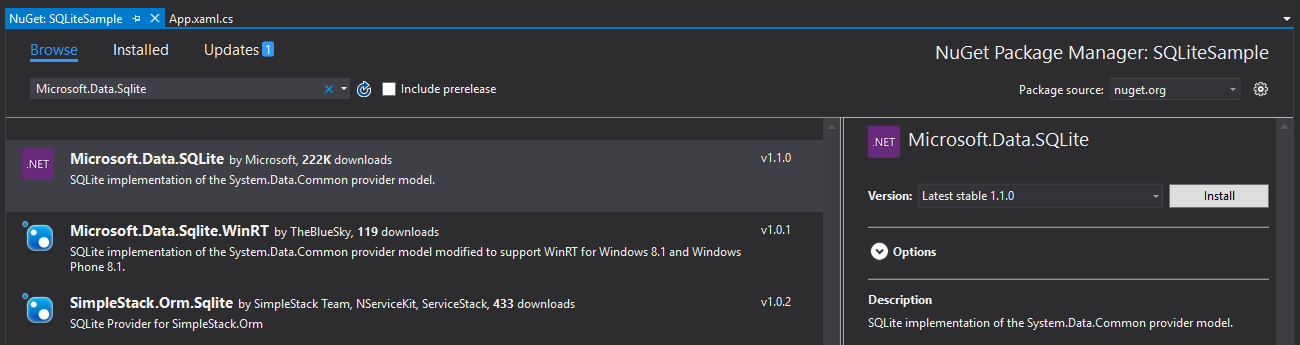
\includegraphics[width=\linewidth]{figures/sqlite_install_microsoft.data.sqlite}
	\caption{\ProgrammingLanguagePackageName{Microsoft.Data.Sqlite}安装界面}
	\label{fig:Microsoft.Data.Sqlite安装界面}
\end{figure}

\subsection{Code}

\subsubsection{Application User Interface}

We’ll start off by making a simple UI for our application so we can see how to add and retrieve entries from our SQLite database.

\begin{lstlisting}[style=HtmlStyle]
<Grid Background="{ThemeResource ApplicationPageBackgroundThemeBrush}">
	<StackPanel>
		<TextBox Name="Input_Box"></TextBox>
		<Button Click="Add_Text">Add</Button>
		<ListView Name="Output">
			<ListView.ItemTemplate>
				<DataTemplate>
					<TextBlock Text="{Binding}"/>
				</DataTemplate>
			</ListView.ItemTemplate>
		</ListView>
	</StackPanel>
</Grid>
\end{lstlisting}

There are three important parts to our application’s interface:

\begin{enumerate}
	\item A text box that allows us to take text from the user.
	\item A button linked to an event for pulling the text and placing it in the SQLite database.
	\item An ItemTemplate to show previous entries in the database.
\end{enumerate}

\subsubsection{Code Behind for Application}
In the App.xaml.cs and MainPage.xaml.cs files generated by Visual Studio, we’ll start by importing the Microsoft.Data.Sqlite namespaces that we’ll be using.

\begin{lstlisting}[style=CSharpStyle]
using Microsoft.Data.Sqlite;
using Microsoft.Data.Sqlite.Internal;
\end{lstlisting}

Then as part of the app constructor, we’ll run a “CREATE TABLE IF NOT EXISTS” command to guarantee that the SQLite .db file and table are created the first time the application is launched.

\begin{lstlisting}[style=CSharpStyle]
public App()
{
	this.InitializeComponent();
	this.Suspending += OnSuspending;
	SqliteEngine.UseWinSqlite3(); //Configuring library to use SDK version of SQLite
	using (SqliteConnection db = new SqliteConnection("Filename=sqliteSample.db"))
	{
		db.Open();
		String tableCommand = @"CREATE TABLE IF NOT EXISTS MyTable (
									Primary_Key INTEGER PRIMARY KEY AUTOINCREMENT, 
									Text_Entry NVARCHAR(2048) NULL)";
		SqliteCommand createTable = new SqliteCommand(tableCommand, db);
		try
		{
			createTable.ExecuteReader();
		}
		catch (SqliteException e)
		{
			//Do nothing
		}
	}
} 
\end{lstlisting}

There are couple of points worth noting with this code:

\begin{enumerate}
	\item We make a call to SqliteEngine.UseWinSqlite3() before making any other SQL calls, which guarantees that the Microsoft.Data.Sqlite framework will use the SDK version of SQLite as opposed to a local version.
	\item We then open a connection to a SQLite .db file. The name of the file passed as a String is your choice, but should be consistent across all SqliteConnection objects. This file is created on the fly the first time it’s called, and is stored in the application’s local data store.
	\item After establishing the connection to the database, we instantiate a SqliteCommand object passing in a String representing the specific command and the SqliteConnection instance, and call execute.
	\item We place the ExecuteReader() call inside a try-catch block. This is because SQLite will always throw a SqliteException whenever it can’t execute the SQL command. Not getting the error confirms that the command went through correctly.
\end{enumerate}

Next, we’ll add code in the View’s code-behind file to handle the button-clicked event. This will take text from the text box and put it into our SQLite database.

\begin{lstlisting}[style=CSharpStyle]
private void Add_Text(object sender, RoutedEventArgs e)
{
	using (SqliteConnection db = new SqliteConnection("Filename=sqliteSample.db"))
	{
		db.Open();

		SqliteCommand insertCommand = new SqliteCommand();
		insertCommand.Connection = db;

		//Use parameterized query to prevent SQL injection attacks
		insertCommand.CommandText = "INSERT INTO MyTable VALUES (NULL, @Entry);";
		insertCommand.Parameters.AddWithValue("@Entry", Input_Box.Text);        

		try
		{
			insertCommand.ExecuteReader();
		}
		catch (SqliteException error)
		{
			//Handle error
			return;
		}
		db.Close();
	}
	Output.ItemsSource = Grab_Entries();
}
\end{lstlisting}

As you can see, this isn’t drastically different than the SQLite code explained in the app’s constructor above. The only major deviation is the use of parameters in the query so as to prevent SQL injection attacks. You will find that commands that make changes to the database (i.e. creating tables, or inserting entries) will mostly follow the same logic.

Finally, we go to the implementation of the Grab\_Entries() method, where we grab all the entries from the Text\_Entry column and fill in the XAML template with this information.

\begin{lstlisting}[style=CSharpStyle]
private List<String> Grab_Entries()
{
	List<String> entries = new List<string>();
	using (SqliteConnection db = new SqliteConnection("Filename=sqliteSample.db"))
	{
		db.Open();
		SqliteCommand selectCommand = new SqliteCommand("SELECT Text_Entry from MyTable", db);
		SqliteDataReader query;
		
		try
		{
			query = selectCommand.ExecuteReader();
		}
		catch(SqliteException error)
		{
			//Handle error
			return entries;
		}
		
		while(query.Read())
		{
			entries.Add(query.GetString(0));
		}
		db.Close();
	}
	return entries;
}
\end{lstlisting}

Here, we take advantage of the SqliteDataReader object returned from the ExecuteReader() method to run through the results and add them to the List we eventually return. There are two methods worth pointing out:

\begin{enumerate}
	\item The Read() method advances through the rows returned back from the executed SQLite command, and returns a boolean based on whether you’ve reached the end of the query or not (True if there are more rows left, and False if you’ve reached the end).
	\item The GetString() method returns the value of the specified column as a String. It takes in one parameter, an int that represents the zero-based column ordinal. There are similar methods like GetDataTime() and GetBoolean() that you can use based on the data type of the column that you are dealing with. 
	\begin{enumerate}
		\item The ordinal parameter isn’t as relevant in this example since we are selecting all the entries in a single column. However, in the case where multiple columns are part of the query, the ordinal represents the column you are pulling from. So if we selected both Primary\_Key and Text\_Entry, then GetString(0) would return the value of Primary\_Key String and GetString(1) would return the value of Text\_Entry as a String.
	\end{enumerate}
\end{enumerate}

And that’s it! You can now build your application and add any text you like into your SQLite database. You can even close and open your application to see that the data persists.

A link to the full code can be found at: \url{https://github.com/Microsoft/windows-developer-blog-samples/tree/master/Samples/SQLiteSample}

\subsubsection{Moving Forward}
There are plenty of additions that you can make to tailor this sample to your needs:
\begin{enumerate}
	\item Adding more tables and more complicated queries.
	\item Providing more sanitation over the text entries to prevent faulty user input.
	\item Communicating with your database in the cloud to propagate information across devices.
	\item And so much more!
\end{enumerate}

\subsection{What about Entity Framework?}

For those developers looking to abstract away particular database details, Microsoft’s Entity Framework provides a great model that lets you work at the “Object” layer as opposed to the database access layer. You can create models for your database using code, or visually define your model in the EF designer. Then Entity Framework makes it super-easy to generate a database from your defined object model. It’s also possible to map your models to existing databases you may have already created.

SQLite is one of many database back-ends that Entity Framework is configured to work with. This documentation provides an example to work from.

\subsection{Conclusion}
From embedded applications for Windows 10 IoT Core to a cache for enterprise relations database server (RDBS) data, SQLite is the premier choice for any application that needs local storage support. SQLite’s server-less and self-contained architecture makes it compact and easy to manage, while its tried and tested API surface coupled with its massive community support provides additional ease of use. And since it ships as part of Windows 10, you can have peace of mind, knowing that you’re always using an up-to-date version of the binary.

As always, please leave any questions in the comments section, and we’ll try our best to answer them. Additional resources are also linked below.

